\documentclass{article}

\usepackage{fancyhdr}
\usepackage{extramarks}
\usepackage{amsmath}
\usepackage{systeme}
\usepackage{parallel}
\usepackage{autoaligne}
\usepackage{amsthm}
\usepackage{amsfonts}
\usepackage{tikz, pgfplots}
\usepackage[plain]{algorithm}
\usepackage{algpseudocode}

\usetikzlibrary{automata,positioning}

%
% Basic Document Settings
%

\topmargin=-0.45in
\evensidemargin=0in
\oddsidemargin=0in
\textwidth=6.5in
\textheight=9.0in
\headsep=0.25in

\linespread{1.1}

\pagestyle{fancy}
\lhead{Solomon Greenberg}
\chead{Section 1.1}
\rhead{MATH 225}
\lfoot{\lastxmark}
\cfoot{\thepage}

\renewcommand\headrulewidth{0.4pt}
\renewcommand\footrulewidth{0.4pt}

\setlength\parindent{0pt}

%
% Create Problem Sections
%


%
% Homework Problem Environment
%
% This environment takes an optional argument. When given, it will adjust the
% problem counter. This is useful for when the problems given for your
% assignment aren't sequential. See the last 3 problems of this template for an
% example.
%

%
% Homework Details
%   - Title
%   - Due date
%   - Class
%   - Section/Time
%   - Instructor
%   - Author
%
%
% Various Helper Commands
%

% Useful for algorithms
\newcommand{\alg}[1]{\textsc{\bfseries \footnotesize #1}}

% For derivatives
\newcommand{\deriv}[1]{\frac{\mathrm{d}}{\mathrm{d}x} (#1)}

% For partial derivatives
\newcommand{\pderiv}[2]{\frac{\partial}{\partial #1} (#2)}

% Integral dx
\newcommand{\dx}{\mathrm{d}x}

% Alias for the Solution section header
\newcommand{\solution}{\textbf{\large Solution}}

% Probability commands: Expectation, Variance, Covariance, Bias
\newcommand{\E}{\mathrm{E}}
\newcommand{\Var}{\mathrm{Var}}
\newcommand{\Cov}{\mathrm{Cov}}
\newcommand{\Bias}{\mathrm{Bias}}

\begin{document}

% \maketitle

% \pagebreak
% \vspace*{\stretch{1.0}}
\large\text{Solomon Greenberg},
\large\text{2017/09/06},
\large\textbf{Homework 1, Section 1.1},
\large\textit{Problems: 7, 11, 12, 13, 16, 24, 26, 39},
\large\textit{Done: 7, 11, 12, 13, 16},

\section*{Problem 7}
\subsection*{Solve: }
$$
\sysdelim||\systeme{
    x + 2y + 3z = 1,
    x + 3y + 4z = 3,
    x + 4y + 5z = 4
}
$$
\subsection*{Solution:}
\begin{equation}
    \begin{array}{rr}
        $I$ \\ $II$ \\ $III$
    \end{array}
    \sysdelim||\systeme{
        x + 2y + 3z = 1 ,
        x + 3y + 4z = 3 ,
        x + 4y + 5z = 4
    }
\end{equation}
\begin{equation}
    \sysdelim||\systeme{
        x + 2y + 3z = 1 ,
        x + 3y + 4z = 3 ,
        x + 4y + 5z = 4
    }
    \begin{array}{rr}
        \longrightarrow \\
        -$I$ \\
        -$I$ \\
    \end{array}
    \sysdelim||\systeme{
        x + 2y + 3z = 1 ,
        y + 4z = 2 ,
        2y + 2z = 3
    }
\end{equation}
\begin{equation}
    \sysdelim||\systeme{
        x + 2y + 3z = 1 ,
        y + 4z = 2 ,
        2y + 2z = 3
    }
    \begin{array}{rr}
        \longrightarrow \\
        -2$III$ \\
        -2$II$ \\
    \end{array}
    \sysdelim||\systeme{
        x + 2y + 3z = 1 ,
        -3y = -4 ,
        -6z = -1
    }
\end{equation}
\begin{equation}
    \sysdelim||\systeme{
        x + 2y + 3z = 1 ,
        -3y = -4 ,
        -6z = -1
    }
    \begin{array}{rr}
        \longrightarrow \\
        \cdot \,{-3} \\
        \cdot \,{-6} \\
    \end{array}
    \sysdelim||\systeme{
        x + 2y + 3z = 1 ,
        y = 12 ,
        z = 6
    }
\end{equation}
\begin{equation}
    \sysdelim||\systeme{
        x + 2y + 3z = 1 ,
        y = 12 ,
        z = 6
    }
    \begin{array}{rr}
        - (2$II$ + 3$III$)\\
        \longrightarrow \\
        \longrightarrow \\
    \end{array}
    \sysdelim||\systeme{
        x = -41,
        y = 12, 
        z = 6
    }
\end{equation}
\begin{equation}
    \sysdelim||\systeme{
        x = -41,
        y = 12, 
        z = 6
    }
\end{equation}

\pagebreak

\section*{Problem 11}
\subsection*{Solve and graph:}
\begin{equation}
    \sysdelim||\systeme{
        x - 2y = 2,
        3x + 5y = 17
    }
\end{equation}
\subsection*{Solution:}
\begin{equation}
    \begin{array}{rr}
        $I$\\$II$
    \end{array}
    \sysdelim||\systeme{
        x - 2y = 2,
        3x + 5y = 17
    }
\end{equation}
\begin{equation}
    \sysdelim||\systeme{
        x - 2y = 2,
        3x + 5y = 17
    }
    \begin{array}{rr}
        \longrightarrow
        \\
        -3$I$
    \end{array}
    \sysdelim||\systeme{
        x - 2y = 2,
        11y = 11
    }
\end{equation}
\begin{equation}
    \sysdelim||\systeme{
        x - 2y = 2,
        11y = 11
    }
    \begin{array}{rr}
        \longrightarrow
        \\
        \cdot \frac{1}{11}
    \end{array}
    \sysdelim||\systeme{
        x - 2y = 2,
        y = 1
    }
\end{equation}
\begin{equation}
    \sysdelim||\systeme{
        x - 2y = 2,
        y = 1
    }
    \begin{array}{rr}
        +2$II$
        \\
        \longrightarrow
    \end{array}
    \sysdelim||\systeme{
        x = 4,
        y = 1
    }
\end{equation}
\begin{equation}
    \sysdelim||\systeme{
        x = 4,
        y = 1
    }
\end{equation}

\begin{center}
    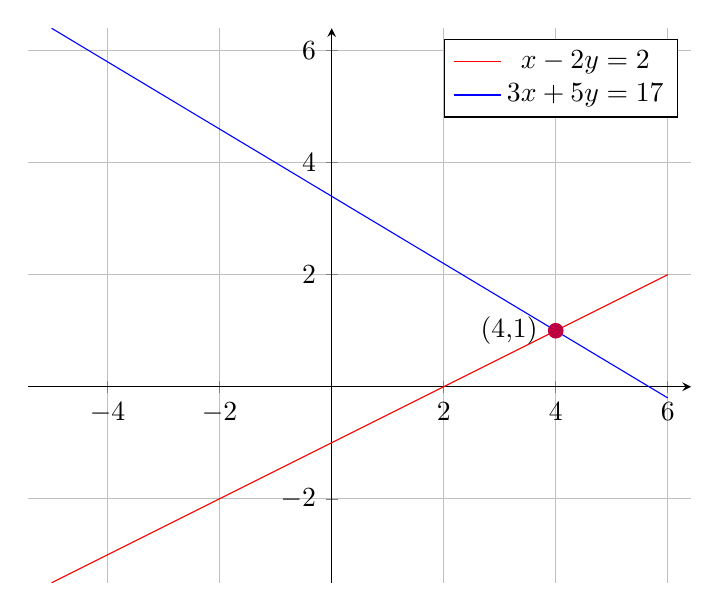
\begin{tikzpicture}
        \begin{axis}[
            axis y line=center,
            axis x line=middle,
            axis equal,
            grid=both,
            % xmax=10,xmin=-10,
            % ymin=-10,ymax=10,
            % xlabel=$x$,ylabel=$y$,
            % xtick={-10,...,10},
            % ytick={-10,...,10},
            width=10cm,
            anchor=center,
            ]
            \addplot [color=red, domain=-5:6]{(x - 2)/2} ;
            \addlegendentry{$x-2y = 2$}
            \addlegendentry{$3x + 5y = 17$}
            \addplot [color=blue, domain=-5:6]{(17-3*x)/5} ;
            \node[label={180:{(4,1)}},color=purple, circle,fill,inner sep=2pt] at (axis cs:4,1) {};
        \end{axis}
        % x - 2y = 2
        % 3x + 5y = 17
        % y = (x - 2)/2
        % 5y = 17 - 3x
        % y = (17-3x)/5
    \end{tikzpicture}
\end{center}

\pagebreak
\section*{Problem 12}
\subsection*{Solve: }
$$
\sysdelim||\systeme{
    x - 2y = 3,
    2x - 4y = 6
}
$$
\subsection*{Solution:}
\begin{equation}
    \sysdelim||\systeme{
        x - 2y = 3,
        2x - 4y = 6
    }
    \begin{array}{rr}
        -$II$
        \\
        -$I$
    \end{array}
    \sysdelim||\systeme{
        0x=0,
        0y=0
    }
\end{equation}
\begin{center}Note: Infinite solutions\end{center}
\begin{center}
    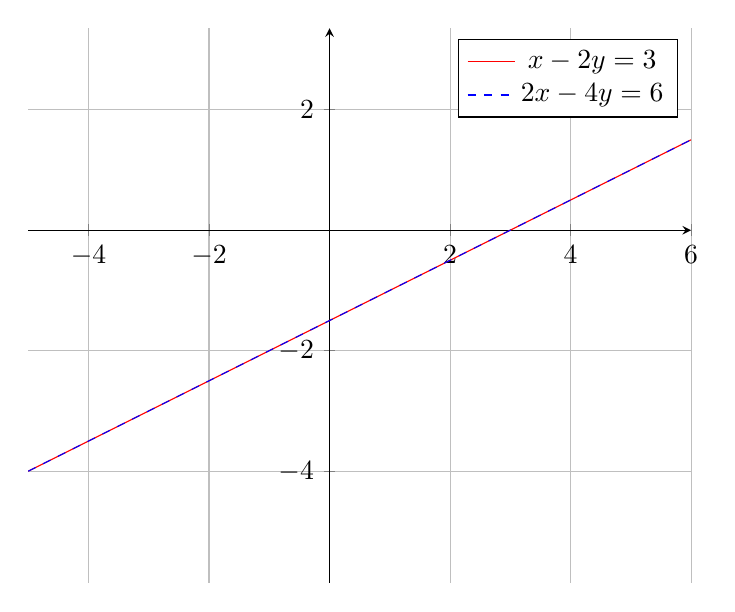
\begin{tikzpicture}
        \begin{axis}[
            axis y line=center,
            axis x line=middle,
            axis equal,
            grid=both,
            % xmax=10,xmin=-10,
            % ymin=-10,ymax=10,
            % xlabel=$x$,ylabel=$y$,
            % xtick={-10,...,10},
            % ytick={-10,...,10},
            width=10cm,
            anchor=center,
            ]
            \addplot [color=red, domain=-5:6]{(x-3)/2} ;
            \addplot [color=blue, domain=-5:6, dashed]{(2*x - 6)/4} ;
            \addlegendentry{$x - 2y = 3$}
            \addlegendentry{$2x - 4y = 6$}
        \end{axis}
        % x - 2y = 2
        % 3x + 5y = 17
        % y = (x - 2)/2
        % 5y = 17 - 3x
        % y = (17-3x)/5
    \end{tikzpicture}
\end{center}

\noindent\makebox[\linewidth]{\rule{16cm}{0.4pt}}

\section*{Problem 13}
\subsection*{Solve: }
$$
\sysdelim||\systeme{
    x - 2y = 3,
    2x - 4y = 8
}
$$
\subsection*{Solution:}
\begin{equation}
    \sysdelim||\systeme{
        x - 2y = 3,
        2x - 4y = 8
    }
    \begin{array}{rr}
        \longrightarrow
        \\
        -2$I$
    \end{array}
    \sysdelim||\systeme{
        x - 2y = 3,
        0 = 2
    }
\end{equation}
\begin{center}Note: No solutions\end{center}
\begin{center}
    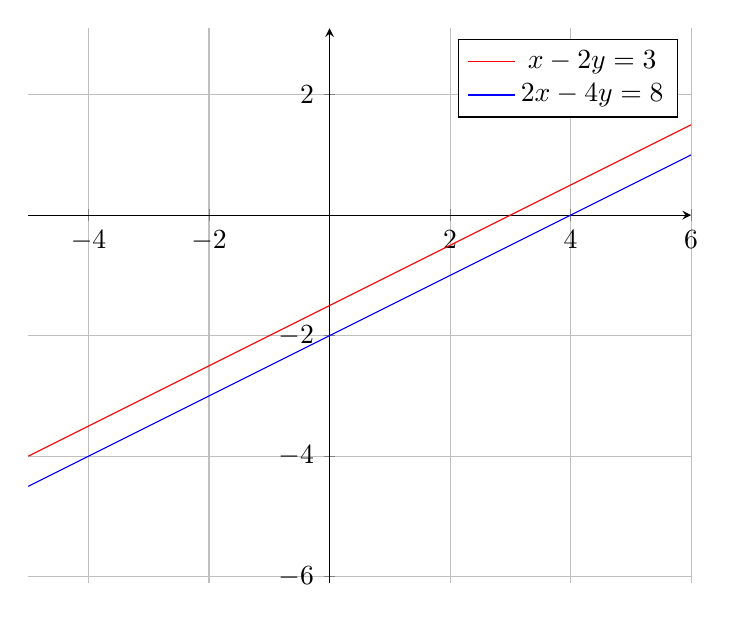
\begin{tikzpicture}
        \begin{axis}[
            axis y line=center,
            axis x line=middle,
            axis equal,
            grid=both,
            % xmax=10,xmin=-10,
            % ymin=-10,ymax=10,
            % xlabel=$x$,ylabel=$y$,
            % xtick={-10,...,10},
            % ytick={-10,...,10},
            width=10cm,
            anchor=center,
            ]
            \addplot [color=red, domain=-5:6]{(x-3)/2} ;
            \addplot [color=blue, domain=-5:6]{(2*x - 8)/4} ;
            \addlegendentry{$x - 2y = 3$}
            \addlegendentry{$2x - 4y = 8$}
        \end{axis}
        % x - 2y = 2
        % 3x + 5y = 17
        % y = (x - 2)/2
        % 5y = 17 - 3x
        % y = (17-3x)/5
    \end{tikzpicture}
\end{center}

\noindent\makebox[\linewidth]{\rule{16cm}{0.4pt}}
\section*{Problem 16}
\subsection*{Solve in terms of intersecting planes: }
$$
\sysdelim||\systeme{
    x + 4y + z = 0,
    4x + 13y + 7z = 0,
    7x + 22y + 13z = 0
}
$$
\subsection*{Solution:}
\begin{equation}
    \sysdelim||\systeme{
        x + 4y + z = 0,
        4x + 13y + 7z = 0,
        7x + 22y + 13z = 0
    }
    \begin{array}{rr}
        \longrightarrow \\
        -7$I$ \\
        -7$I$ \\
    \end{array}
    \sysdelim||\systeme{
        x + 4y + z = 0,
        -3x - 15y = 0,
        -6y + 6z = 0
    }
\end{equation}
\begin{equation}
    \sysdelim||\systeme{
        x + 4y + z = 0,
        -3x - 15y = 0,
        -6y + 6z = 0
    }
    \begin{array}{rr}
        \longrightarrow \\
        \cdot \frac{-1}{3} \\
        \cdot \frac{-1}{6} \\
    \end{array}
    \sysdelim||\systeme{
        x + 4y + z = 0,
        x + 5y = 0,
        y - z = 0
    }
\end{equation}
\begin{equation}
    \sysdelim||\systeme{
        x + 4y + z = 0,
        x + 5y = 0,
        y - z = 0
    }
    \begin{array}{rr}
        \longrightarrow \\
        -$III$\\
        \longrightarrow \\
    \end{array}
    \sysdelim||\systeme{
        x + 4y + z = 0,
        x + 4y + z = 0,
        y - z = 0
    }
\end{equation}
\begin{equation}
    \sysdelim||\systeme{
        x + 4y + z = 0,
        x + 4y + z = 0,
        y - z = 0
    }
    \begin{array}{rr}
        \longrightarrow \\
        -$I$\\
        \longrightarrow \\
    \end{array}
    \sysdelim||\systeme{
        x + 4y + z = 0,
        0x + 0y + 0z = 0,
        y - z = 0
    }
\end{equation}
\begin{equation}
    \sysdelim||\systeme{
        x + 4y + z = 0,
        y - z = 0
    }
\end{equation}
\begin{equation}
    \sysdelim||\systeme{
        x = - 5z,
        y = z
    }
\end{equation}
\begin{equation}
    \systeme{
        x = - 5t,
        y = t
    }
\end{equation}
\noindent\makebox[\linewidth]{\rule{16cm}{0.4pt}}
\section*{Problem 24}
\subsection*{Setup: }
Let $D_a$ represent the yearly demand for product A, in millions of dollars\\
Let $D_b$ represent the yearly demand for product B, in millions of dollars\\
Let $R_a$ represent the required \$ of product A to produce \$1 of B\\
Let $R_b$ represent the required \$ of product B to produce \$1 of A
\subsection*{Solve: }
$$
\sysdelim||\systeme{
    a - R_b b = D_a,
    -R_a a + b = D_b
}
$$
\subsection*{Solution:}
\begin{equation}
    \sysdelim||\systeme{
        a - 0.1b = 1000,
        -0.2a + b = 780
    }
    \begin{array}{rr}
        \cdot 10\\
        \longrightarrow \\
    \end{array}
    \sysdelim||\systeme{
        10a - b = 10000,
        -0.2a + b = 780
    }
\end{equation}
\begin{equation}
    \sysdelim||\systeme{
        10a - b = 10000,
        -0.2a + b = 780
    }
    \begin{array}{rr}
        + $II$\\
        \longrightarrow \\
    \end{array}
    \sysdelim||\systeme{
        9.8a = 10780,
        -0.2a + b = 780
    }
\end{equation}
\begin{equation}
    \sysdelim||\systeme{
        9.8a = 10780,
        -0.2a + b = 780
    }
    \begin{array}{rr}
        \cdot \frac{1}{9.8}\\
        \cdot 5\\
    \end{array}
    \sysdelim||\systeme{
        a = 1100,
        -a + 5b = 3900
    }
\end{equation}
\begin{equation}
    \sysdelim||\systeme{
        a = 1100,
        -a + 5b = 3900
    }
    \begin{array}{rr}
        \longrightarrow \\
        +$I$\\
    \end{array}
    \sysdelim||\systeme{
        a = 1100,
        b = 1000
    }
\end{equation}
\begin{equation}
    \sysdelim||\systeme{
        a = 1100,
        b = 1000
    }
\end{equation}
\begin{center}Required output of product A: \$1100 million/year\\
Required output of product B: \$1000 million/year \end{center}


\end{document}
